\documentclass[pdf, 9pt]{beamer}
\mode<presentation>{}
\usetheme{Darmstadt}
\usepackage{caption}
\setbeamertemplate{caption}[numbered]
\usepackage{multirow}
\usepackage{graphics}
\usepackage{svg}
\usepackage{hyperref}

\newcommand\blfootnote[1]{%
	\begingroup
	\renewcommand\thefootnote{}\footnote{#1}%
	\addtocounter{footnote}{-1}%
	\endgroup
}

%% preamble
\title{Classification of Fever Patterns using Deep Learning}
\subtitle{Under the guidance of Dr. Sumam David}
\author{Anirudh Prabhakaran}
\institute{National Institute of Technology, Karnataka}

\begin{document}
	
	%% title frame
	\begin{frame}
		\titlepage
	\end{frame}
	
	\section{Problem Statement and Objectives}
	\begin{frame}
		\frametitle{Problem Statement and Objectives}
		\begin{itemize}
			\item Problem Statement
			\begin{itemize}
				\item Use deep learning algorithms on temperature data of patients to classify diseases like TB, dengue, etc.
			\end{itemize}
			\item Objectives
			\begin{itemize}
				\item Classify diseases faster and with higher accuracy.
				\item Find patterns in temperature data characteristic of various disease.
			\end{itemize}
		\end{itemize}
		\blfootnote{All code for the project can be found at \href{https://github.com/anirudhprabhakaran3/diagnosis-temperature-data}{\underline{this GitHub repository}}.}
	\end{frame}
	
	\section{Data}
	\begin{frame}
		\frametitle{Data}
		\begin{itemize}
			\item Dataset consists of temperature data for every minute a day (1440 data points) for 185 patients.
			\item We consider only 4 classes - Dengue, Non-Infectious Diseases, Non-tubercular Bacterial Infection, Tuberculosis.
			\item Total 144 records have been chosen.
			\item Train - test split of 80\% - 20\%
			\item Training records: 115
			\item Testing records: 29
		\end{itemize}
	\end{frame}
	
	\begin{frame}
		\frametitle{Data}
		\begin{table}[]
			\begin{tabular}{|c|c|}
				\hline
				\textbf{Disease}                   & \textbf{Counts} \\ \hline
				Dengue                             & 47              \\
				Leptospirosis                      & 15              \\
				Malaria                            & 16              \\
				Malignancy                         & 7               \\
				Non-Infectious Diseases            & 28              \\
				Non-Tubercular Bacterial Infection & 37              \\
				Pyogenic Sepsis                    & 2               \\
				Thyroiditis                        & 1               \\
				Tuberculosis                       & 32              \\ \hline
			\end{tabular}
			\captionof{table}{Dataset Description}
		\end{table}
	\end{frame}
	
	\begin{frame}
		\frametitle{Data}
		\begin{figure}
			\centering
			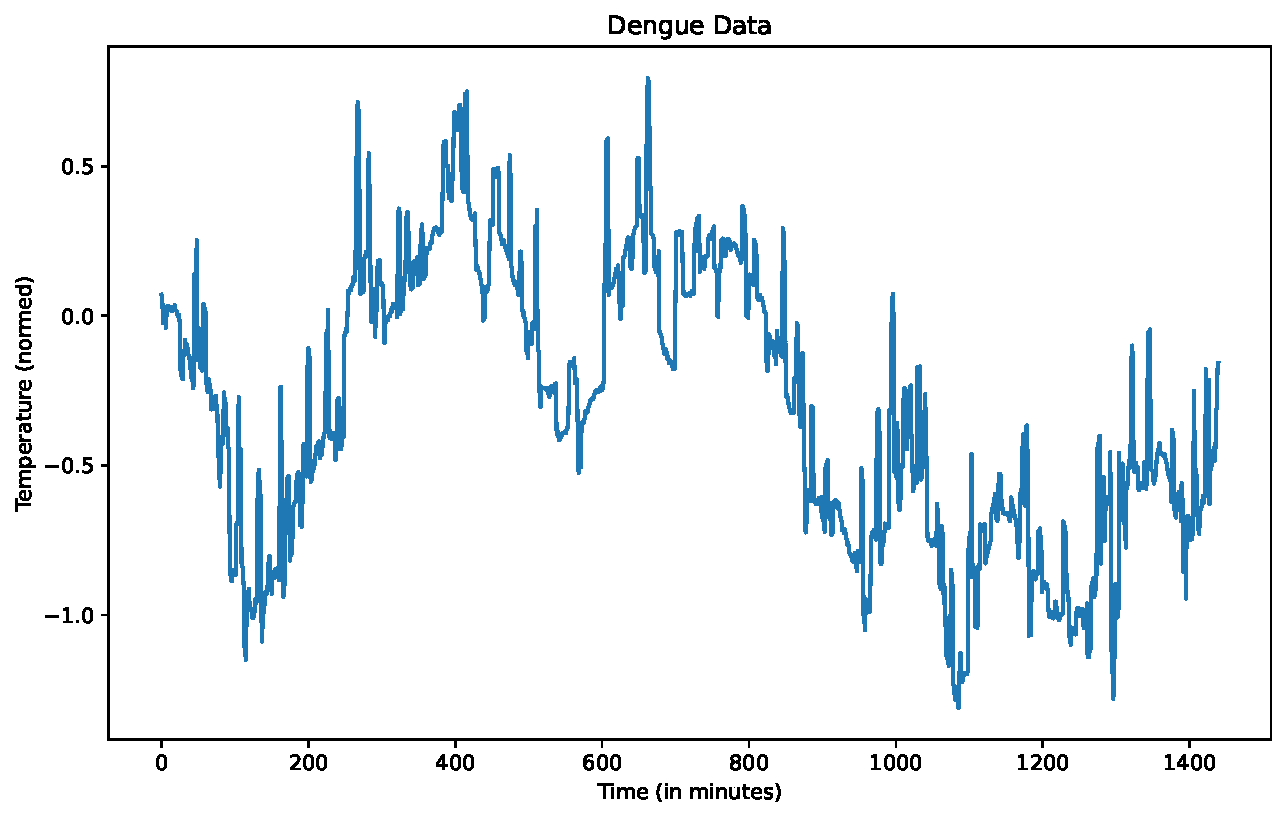
\includegraphics[width=0.4\linewidth]{figures/dengue_data.pdf}
			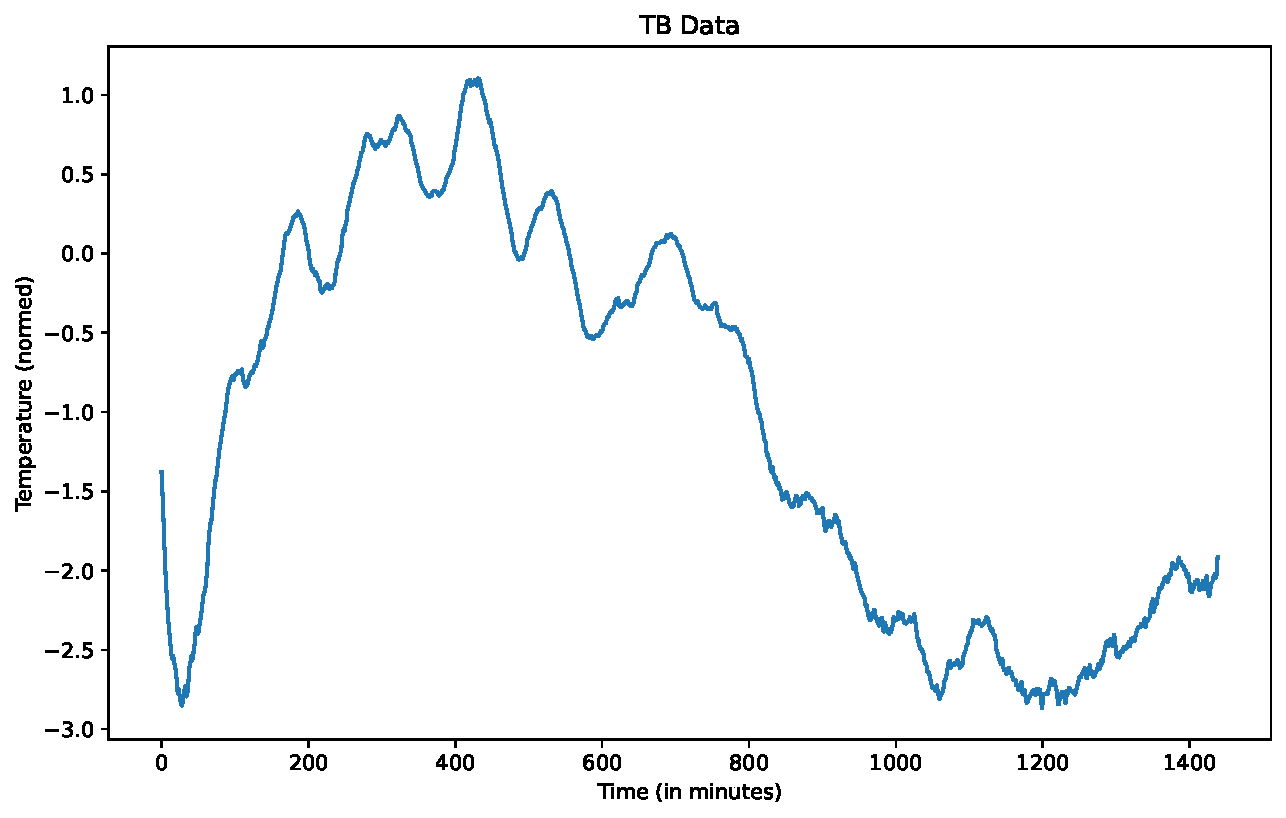
\includegraphics[width=0.4\linewidth]{figures/tb_data.pdf}
			\caption{Temperature visualization for Dengue and Tuberculosis}
		\end{figure}
		
		\begin{figure}
			\centering
			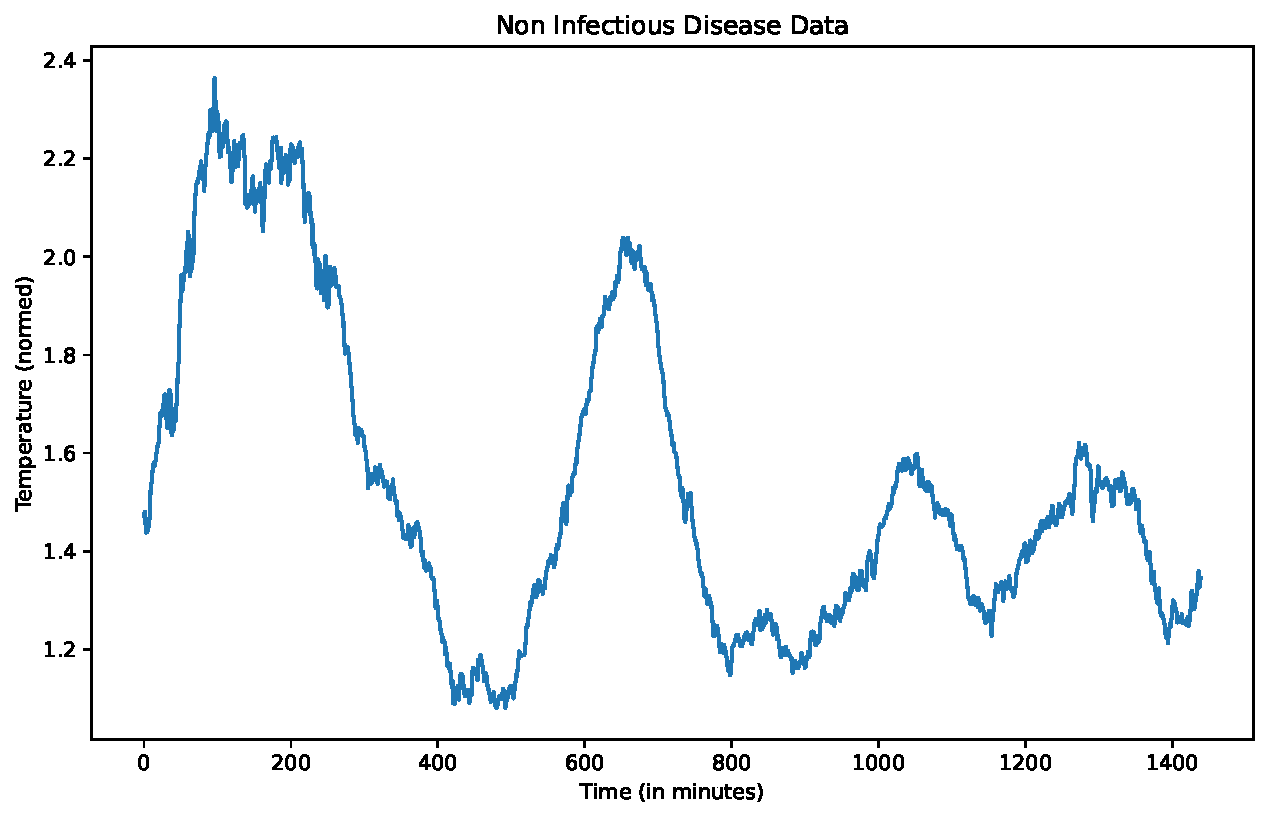
\includegraphics[width=0.4\linewidth]{figures/non_infectious_data.pdf}
			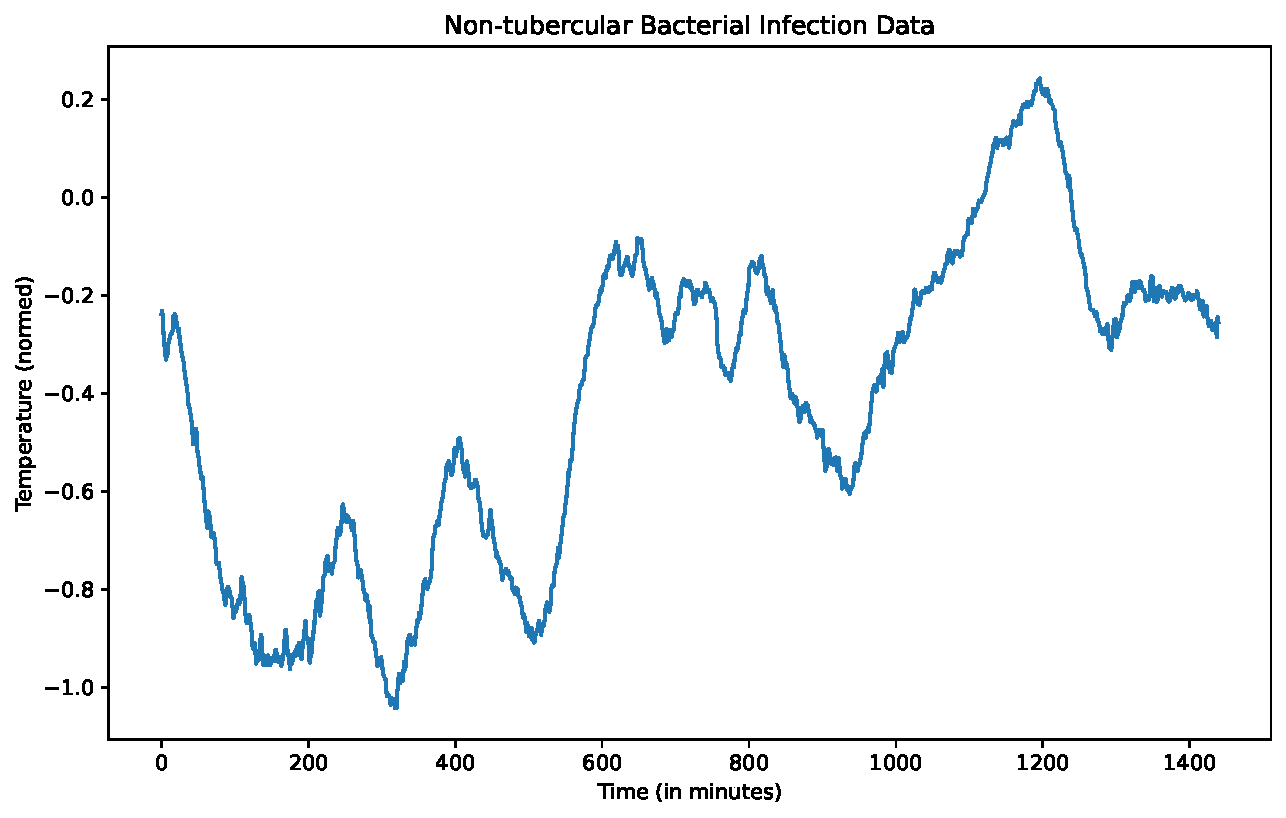
\includegraphics[width=0.4\linewidth]{figures/non_tubercular_data.pdf}
			\caption{Temperature visualization for Non-Infectious Diseases and Non-Tubercular Bacterial Infection}
		\end{figure}
	\end{frame}
	
	\section{Models}
	\begin{frame}
		\frametitle{Models}
		\begin{table}[]
			\centering
			\begin{tabular}{|c|c|c|}
				\hline
				\textbf{Model Name}                   & \textbf{\# of params} & \textbf{Model Size (MB)} \\ \hline
				Multi Layer Perceptron                & 5,764                 & 0.07                     \\
				Three Layer NN (with/without dropout) & 2,033,476             & 8.28                     \\
				1D CNN                                & 123,012               & 8.39                     \\
				1D Two Block CNN                      & 53,572                & 10.72                    \\
				1D Three Block CNN                    & 63,428                & 14.22                    \\
				1 Layer RNN                           & 4,548                 & 5.96                     \\
				2 Layer RNN                           & 12,868                & 6.00                     \\
				3 Layer RNN                           & 21,188                & 6.03                     \\
				LSTM                                  & 83,972                & 6.28                     \\ \hline
			\end{tabular}
			\captionof{table}{Model Details}\label{model_details}
		\end{table}
	\end{frame}
	
	\section{Results}
	\begin{frame}
		\frametitle{Training Results}
		
		\begin{table}[]
			\centering
			\resizebox{\columnwidth}{!}{%
			\begin{tabular}{|c|c|c|c|c|c|c|}
				\hline
				\textbf{Model Name}                             & \textbf{Optimizer} & \textbf{Loss}  & \textbf{Accuracy} & \textbf{Precision} & \textbf{Recall} & \textbf{F1 Score} \\ \hline
				\multirow{2}{*}{Multi Layer Perceptron}         & SGD                & 1.072          & 0.662             & 0.691              & 0.662           & 0.657             \\
				& Adam & 1.019 & 0.701 & 0.721 & 0.701 & 0.702 \\ \hline
				\multirow{2}{*}{Three Layer NN without Dropout} & SGD                & \textbf{0.847} & 0.718             & 0.744              & 0.718           & 0.685             \\
				& Adam & 1.443 & 0.330 & 0.365 & 0.330 & 0.256 \\ \hline
				\multirow{2}{*}{Three Layer NN with Dropout}    & SGD                & 0.910          & 0.587             & 0.505              & 0.587           & 0.500             \\
				& Adam & 1.423 & 0.361 & 0.269 & 0.361 & 0.243 \\ \hline
				\multirow{2}{*}{1D CNN}           & SGD  & 1.033 & 0.679 & 0.697 & 0.679 & 0.683 \\
				& Adam & 1.108 & 0.585 & 0.582 & 0.585 & 0.575 \\ \hline
				\multirow{2}{*}{1D Two Block CNN} & SGD  & 0.909 & 0.780 & 0.784 & 0.780 & 0.780 \\
				& Adam & 0.863 & 0.799 & 0.806 & 0.799 & 0.800 \\ \hline
				\multirow{2}{*}{1D Three Block CNN}             & SGD                & 0.873          & \textbf{0.812}    & \textbf{0.814}     & \textbf{0.812}  & \textbf{0.811}    \\
				& Adam & 1.001 & 0.746 & 0.755 & 0.746 & 0.747 \\ \hline
				\multirow{2}{*}{1 Layer RNN}      & SGD  & 1.378 & 0.284 & 0.145 & 0.284 & 0.164 \\
				& Adam & 1.355 & 0.306 & 0.220 & 0.306 & 0.231 \\ \hline
				\multirow{2}{*}{2 Layer RNN}      & SGD  & 1.366 & 0.311 & 0.137 & 0.311 & 0.166 \\
				& Adam & 1.331 & 0.342 & 0.284 & 0.34  & 0.292 \\ \hline
				\multirow{2}{*}{3 Layer RNN}      & SGD  & 1.370 & 0.325 & 0.149 & 0.325 & 0.166 \\
				& Adam & 1.347 & 0.356 & 0.305 & 0.356 & 0.279 \\ \hline
				\multirow{2}{*}{LSTM}             & SGD  & 1.368 & 0.321 & 0.103 & 0.321 & 0.15  \\
				& Adam & 1.382 & 0.350 & 0.216 & 0.350 & 0.242 \\ \hline
			\end{tabular}%
			}
			\captionof{table}{Model Training Metrics}\label{model_training_metrics}
		\end{table}
	\end{frame}
	
	\begin{frame}
		\frametitle{Testing Results}
		
		\begin{table}[]
			\resizebox{\columnwidth}{!}{%
			\begin{tabular}{|c|c|c|c|c|c|c|}
				\hline
				\textbf{Model Name} & \textbf{Optimizer} & \textbf{Loss} & \textbf{Accuracy} & \textbf{Precision} & \textbf{Recall} & \textbf{F1 Score} \\ \hline
				\multirow{2}{*}{Multi Layer Perceptron}         & SGD  & 1.411          & 0.344          & 0.363          & 0.344          & 0.337          \\
				& Adam & 1.401          & 0.310          & 0.324          & 0.310          & 0.311          \\ \hline
				\multirow{2}{*}{Three Layer NN without Dropout} & SGD  & 1.363          & 0.379          & 0.445          & 0.379          & 0.324          \\
				& Adam & 1.398          & 0.344          & 0.748          & 0.344          & 0.409          \\ \hline
				\multirow{2}{*}{Three Layer NN with Dropout}    & SGD  & \textbf{1.288} & 0.413          & 0.551          & 0.413          & 0.459          \\
				& Adam & 1.329          & 0.413          & \textbf{1.000} & 0.413          & 0.585          \\ \hline
				\multirow{2}{*}{1D CNN}                         & SGD  & 1.369          & 0.344          & 0.340          & 0.344          & 0.337          \\
				& Adam & 1.369          & 0.379          & 0.393          & 0.379          & 0.369          \\ \hline
				\multirow{2}{*}{1D Two Block CNN}               & SGD  & 1.453          & 0.241          & 0.476          & 0.241          & 0.260          \\
				& Adam & 1.426          & 0.275          & 0.384          & 0.275          & 0.286          \\ \hline
				\multirow{2}{*}{1D Three Block CNN}             & SGD  & 1.457          & 0.275          & 0.521          & 0.275          & 0.342          \\
				& Adam & 1.416          & 0.310          & 0.439          & 0.310          & 0.360          \\ \hline
				\multirow{2}{*}{1 Layer RNN}                    & SGD  & 1.338          & \textbf{0.448} & 0.635          & \textbf{0.448} & \textbf{0.524} \\
				& Adam & 1.373          & 0.310          & 0.366          & 0.310          & 0.334          \\ \hline
				\multirow{2}{*}{2 Layer RNN}                    & SGD  & 1.352          & 0.413          & 0.770          & 0.413          & 0.534          \\
				& Adam & 1.372          & 0.275          & 0.351          & 0.275          & 0.306          \\ \hline
				\multirow{2}{*}{3 Layer RNN}                    & SGD  & 1.356          & 0.344          & 0.896          & 0.344          & 0.498          \\
				& Adam & 1.413          & 0.344          & 0.896          & 0.344          & 0.498          \\ \hline
				\multirow{2}{*}{LSTM}                           & SGD  & 1.367          & 0.344          & \textbf{1.000} & 0.344          & 0.512          \\
				& Adam & 1.460          & 0.206          & 0.455          & 0.206          & 0.283          \\ \hline
			\end{tabular}%
		}
		\captionof{table}{Model Testing Metrics}\label{model_testing_metrics}
		\end{table}
	\end{frame}
	
	\section{Future Steps}
	\begin{frame}
		\frametitle{Future Steps}
		\begin{itemize}
			\item Run GradCAM and other explainable AI tools.
			\item Run models on other available open-source temperature datasets to check performance on OOD data.
			\item Optimize model to work with less data point, rather than entire 1440 data points.
		\end{itemize}
	\end{frame}
	
	\section{References}
	\begin{frame}
		\frametitle{References}
		\bibliographystyle{abbrv}
		\bibliography{refs}
		\nocite{*}
	\end{frame}
	
\end{document}